\chapter{Modelos clásicos}

En este capítulo nos centraremos en dos de los modelos mencionados en \cite{mateModelsInPopulationAndEpidemiology} por  Brauer y Castillo: los modelos SIS y SIR, en los que se considera la muerte causada por la enfermedad. Analizaremos la estabilidad y realizaremos una implementación que nos permita conocer las soluciones discretas de las ecuaciones diferenciales que describen cada modelo.

Para estudiar la dinámica de cada modelo nos apoyaremos del trabajo realizado en \cite{diego2010}, en donde se describen los análisis para modelos SIR con población de tamaño constante y normalizado, por lo que tendremos que realizar algunos ajustes en la escritura de los modelos contemplados en \cite{mateModelsInPopulationAndEpidemiology}.

\section{El modelo SIS}

El modelo SIS considera 2 posibles estados, susceptibles (S) e infectados (I). Las variaciones entre los estados vienen dadas por los nuevos contagios y los individuos que se recuperan de la enfermedad. Adicionalmente, cada estado se ve afectado por los parámetros que describen la natalidad/mortalidad y la muerte a cauda de la enfermedad. 

Los diferentes estados del modelo se pueden apreciar en el siguiente diagrama:

\begin{figure}[h]
  \centering
    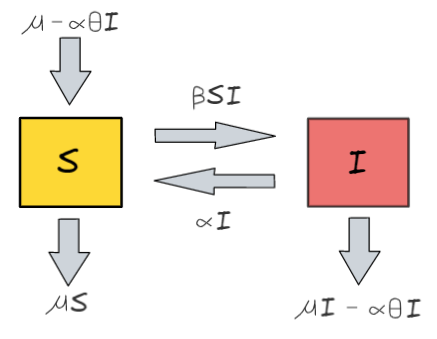
\includegraphics[width=0.4\textwidth]{Imagenes/SIS_compartimientos.PNG}
  \caption{Diagrama de compartimientos para el modelo SIS}
  \label{fig:ClasicSIS}
\end{figure}

Es importante recordar que trabajaremos sobre una población de tamaño constante y normalizado, por lo que $S + I = 1$ y en consecuencia $S' + I' = 0$.

Normalmente cuando se habla de modelos epidemiológicos con muerte por enfermedad se consideran 4 parámetros: 

\begin{itemize}
    \item La \textbf{tasa de infección $\beta$}, que representa la probabilidad que tiene un individuo susceptible de adquirir la enfermedad luego de un contagio con un infectado.
    \item La \textbf{tasa de recuperación $\alpha$}, que podemos entender como la probabilidad de que un infectado se recupere de la enfermedad.
    \item La \textbf{tasa de natalidad/mortalidad $\mu$}, que en el caso de los modelos clásicos se considera igual. La natalidad nos indica la cantidad de individuos que ingresan al espacio y la mortalidad representa los individuos que fallecen por causas ajenas a la enfermedad.
    \item La \textbf{tasa de muerte por enfermedad $\theta$}, que nos indica la probabilidad que tiene un infectado de fallecer a causa de la enfermedad.
\end{itemize}

Podemos describir el modelo a partir de un sistema de ecuaciones diferenciales como sigue:

\begin{equation}\label{eq:ModelSIS}
\left\{
\begin{array}{l}
S' = \mu(1 - S) + (1 - \theta)\alpha I - \beta S I \\
I' = \beta S I - (1 - \theta)\alpha I - \mu I
\end{array}
\right.
\end{equation}

Para determinar los escenarios bajo los cuales una enfermedad es endémica debemos calcular el valor de $R_0$ para nuestro sistema de ecuaciones diferenciales (\ref{eq:ModelSIS}). Recuerde que para determinar el valor de $R_0$ se considera una población completamente susceptible, es decir, $S=1$ y $I=0$.

Observe que los nuevos infectados vienen dados por el término $\beta S$, con lo cual definimos $b(t) = \beta S = \beta$. Por otro lado, los flujos que determinan la salida del estado de infección de los individuos viene dado por los términos $-\alpha(1-\theta)I-\mu I$, de modo que si llamamos $I(t)$ a la cantidad de individuos infectados que permanecieron infectados desde el momento 0, tenemos

\begin{equation}
\frac{dI}{dt} = -\alpha(1-\theta)I-\mu I
\end{equation}

Donde al usar el método de separación de variables obtenemos

\begin{equation}\label{eq:I-SIS}
I(t) = I(0)e^{-(\alpha(1-\theta)+\mu)t}
\end{equation}

De ese modo, podemos afirmar que la proporción de individuos que permanecen infectados hasta un tiempo $t$ viene dado por $e^{-(\alpha(1-\theta)+\mu)t}$, con lo cual $F(t)=e^{-(\alpha(1-\theta)+\mu)t}$. Finalmente, al reemplazar en (\ref{eq:R0}) obtenemos:

\begin{align*}
R_0 &= \lim_{T\to\infty}\int_0^T b(t)F(t) dt \\
&= \lim_{T\to\infty}\int_0^T \beta e^{-(\alpha(1-\theta)+\mu)t} dt\\
&= \frac{\beta}{\alpha(1-\theta)+\mu}
\end{align*}

\underline{\textit{Observación:}} De la ecuación (\ref{eq:I-SIS}) podemos afirmar que la cantidad de individuos infectados tiende a cero cuando $t$ tiende a infinito.

\subsection{Análisis de estabilidad}

Para analizar la estabilidad de nuestro modelo SIS debemos conocer sus puntos de equilibrio. Al anular ambas derivadas nos damos cuenta de que están dados por 

$$P_0=(S_a,I_a)=(1,0), P_1=(S_b,I_b)=\left(\frac{\alpha(1-\theta)+\mu}{\beta},\frac{\beta-\alpha(1-\theta)-\mu}{\beta}\right)$$

Veamos que los puntos de equilibrio satisfacen las condiciones de ser positivos y menores o iguales a 1:

En el caso de $P_0$ la verificación es trivial. Por otro lado, para el caso de $P_1$ observe que 

$$0\leq\alpha(1-\theta)+\mu\leq\beta \longrightarrow \frac{\alpha(1-\theta)+\mu}{\beta}\text{, }\frac{\beta+\alpha(1-\theta)+\mu}{\beta}\geq0$$

Si dividimos la expresión del lado izquierdo por $\beta$ obtenemos

$$0\leq \frac{\alpha(1-\theta)+\mu}{\beta}\leq1$$

De donde podemos afirmar que 

$$1-\frac{\alpha(1-\theta)+\mu}{\beta}\leq1 \longrightarrow \frac{\beta-\alpha(1-\theta)-\mu}{\beta}\leq1$$

De donde podemos concluir que ambos puntos de equilibrio cumplen las condiciones de tener coordenadas positivas y menores que la unidad.

Es momento de determinar los comportamientos que describen ambos puntos, $P_0$ y $P_1$. Consideremos el jacobiano de nuestro modelo:

$$|A-\lambda I|=
\left|\begin{array}{cc}
-\mu-\beta I-\lambda & \lambda(1-\theta)-\beta S \\
\beta I & \beta S-\alpha(1-\theta)-\mu-\lambda
\end{array}\right|$$

Si evaluamos en $P_0$ obtendremos los valores propios

$$\left\{\begin{array}{l}\lambda=-\mu \\
\lambda=\beta-\alpha(1-\theta)-\mu\end{array}\right.$$

Con lo cual, podemos afirmar que si $R_0>1$, $P_0$ se comportará como un punto de silla y por otro lado, si $R_0<1$ estaremos ante un nodo estable. Para el caso de $P_1$ tendremos un comportamiento tipo sumidero dado que $\lambda=0,\lambda=-\mu$ son los valores propios asociados a $P_1$.

\subsection{Estudio numérico}

Para representar las soluciones del sistema de ecuaciones diferenciales que describe el modelo SIS usaremos el método de Euler, el cual se implementó en el módulo: "\textit{CompartmentalModelsInEDOS}".

De manera general, dadas unas condiciones iniciales $S(0)=S_0,I(0)=I_0$ aplicamos el método de Euler a partir de la siguiente expresión

$$\left\{\begin{array}{l}
S_{t+1} = S_t + h\cdot(\mu(1 - S_t) + (1 - \theta)\alpha I_t - \beta S_t I_t ) \\
I_{t+1} = I_t + h\cdot(\beta S_t I_t - (1 - \theta)\alpha I_t - \mu I_t)
\end{array}\right.$$

\begin{itemize}
    \item Consideremos por ejemplo una enfermedad en la que la tasa de recuperación $\alpha$ es del $0.2$ y su tasa de infección es de $\beta=0.5$ con una tasa de letalidad de $\theta=0.4$. La tasa de natalidad para nuestra población será de $\mu=\frac{1}{75\cdot365}$, es decir, una esperanza de vida de $75$ años.
    
    \begin{figure}[h]
      \centering
        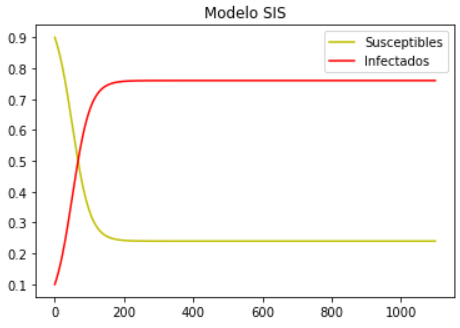
\includegraphics[width=0.4\textwidth]{Imagenes/ex1SIS.PNG}
      \caption{Evolución de la enfermedad en 1100 días con $S_0=0.9,I_0=0.1$ y $h=0.1$.}
      \label{fig:ex1SIS}
    \end{figure}
\end{itemize}

\section{El modelo SIR}

Para este modelo se considera el estado de inmunidad frente a la enfermedad R. A diferencia del modelo SIS, en el modelo SIR no hay una interacción del estado I al estado S, ya que se supone que los individuos que se recuperen de la enfermedad no podrán volver a contraerla, por lo que pasaran al estado R. 

En el siguiente diagrama se pueden apreciar las interacciones para los estados del modelo:

\begin{figure}[h]
  \centering
    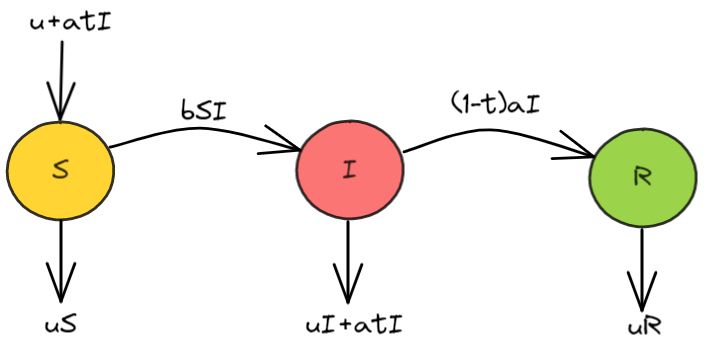
\includegraphics[width=0.7\textwidth]{Imagenes/SIR_compartimientos.PNG}
  \caption{Diagrama de compartimientos para el modelo SIR}
  \label{fig:ClasicSIR}
\end{figure}

De ese modo, el sistema de ecuaciones diferenciales que describe las interacciones entre estados viene dado por la siguiente ecuación:

\begin{equation}\label{eq:SIR}
\left\{
\begin{array}{l}
S' = \mu(1 - S) + \alpha\theta I - \beta S I \\
I' = \beta S I - \mu I - \theta\alpha I - (1 - \theta)\alpha I = \beta S I - \alpha I - \mu I \\
R' = \alpha I - \alpha\theta I - \mu R
\end{array}
\right.
\end{equation}

En este caso, la ecuación diferencial que describirá la cantidad de individuos infectados desde el momento 0 viene dada por:

\begin{equation}\label{eq:ISIR}
    \frac{dI}{dt}=-\mu I - \alpha I \longrightarrow I(t)=I(0)e^{-(\alpha+\mu)t}
\end{equation}

Con lo que definimos $F(t)=e^{-(\alpha+\mu)t}$. Por otra parte, la función $b(t)$ estará definida de la misma manera que en el modelo SIS debido a la manera en la que se describe el modelo. Así, al reemplazar en (\ref{eq:R0}):

\begin{align*}
R_0 &= \int_0^\infty b(t)F(t) dt \\
&= \lim_{T\to\infty} \int_0^T b(t)F(t) dt \\
&= \frac{\beta}{\alpha+\mu}
\end{align*}

\underline{\textit{Observación:}} De acuerdo con la ecuación \ref{eq:ISIR}, la población de infectada tendera a cero cuando $t$ tienda a infinito.

\subsection{Análisis de estabilidad}

Al igualar a cero las derivadas del sistema de ecuaciones \ref{eq:SIR} obtenemos los puntos de equilibrio:

$$\begin{array}{cc}
P_0=(S_a,I_a,R_a)=(1,0,0) & P_1=(S_b,I_b,R_b)=\left(\frac{\alpha+\mu}{\beta},\frac{\mu(\beta-\alpha-\mu)}{\beta(\mu+(1-\theta)\alpha)},\frac{(1-\theta)\alpha(\beta-\alpha-\mu)}{\beta(\mu+(1-\theta)\alpha)}\right)
\end{array}$$

Veamos que las coordenadas de ambos puntos cumplen las condiciones de ser positivos y menores o iguales que uno: 

En el caso de $P_0$ se cumple de manera trivial. Por otro lado, como $\alpha,\beta,\theta$ y $\mu$ son valores positivos podemos afirmar que $S_b>0$, para $I_b$ y $R_b$ observe que 

$$\begin{array}{ccc}
\frac{\mu(\beta-\alpha-\mu)}{\beta(\mu+(1-\theta)\alpha)},\frac{(1-\theta)\alpha(\beta-\alpha-\mu)}{\beta(\mu+(1-\theta)\alpha)}>0 & \text{, si} & \beta-\alpha-\mu>0
\end{array}$$

De la ecuación anterior podemos afirmar que 

$$\beta-\alpha-\mu>0\longrightarrow1>\frac{\alpha+\mu}{\beta}$$

Además, como ya sabemos que se trata de un valor positivo podemos deducir que 

\begin{align*}
1&>1-\frac{\alpha+\mu}{\beta} \\
&= \frac{(\beta-\alpha-\mu)(\mu+(1-\theta)\alpha)}{\beta(\mu+(1-\theta)\alpha)}\\
&= \frac{\mu(\beta-\alpha-\mu)}{\beta(\mu+(1-\theta)\alpha)}+\frac{(1-\theta)\alpha(\beta-\alpha-\mu)}{\beta(\mu+(1-\theta)\alpha)}
\end{align*}

Con lo cual,

$$\frac{\mu(\beta-\alpha-\mu)}{\beta(\mu+(1-\theta)\alpha)},\frac{(1-\theta)\alpha(\beta-\alpha-\mu)}{\beta(\mu+(1-\theta)\alpha)}<1$$

Hemos demostrado que ambos puntos de equilibrio cumplen con las condiciones de tener coordenadas positivas y menores a la unidad. Ahora analizaremos la estabilidad de nuestro modelo SIR, consideremos el jacobiano de nuestro sistema de ecuaciones diferenciales:

$$|A-\lambda I|=(-\mu-\lambda)
\left|\begin{array}{cc}
-\beta I-\mu-\lambda & -\beta S+\theta\alpha\\
\beta I & \beta S-\alpha-\mu -\lambda
\end{array}\right|$$

Si evaluamos en el punto $P_1$, podemos identificar un comportamiento de tipo silla si $\beta-\alpha-\mu>0$, en caso contrario nos encontraremos ante un nodo estable.

Si tomamos ahora el punto $P_2$ y observamos los valores propios 

$$\left\{\begin{array}{l}
\lambda=-\mu\\
\lambda=-\frac{1}{2}\frac{\mu\beta-\mu\theta\alpha+\sqrt{(\mu\beta-\mu\theta\alpha)^2-4\mu(\beta-\alpha-\mu)(\alpha+\mu-\theta\alpha)^2}}{\alpha+\mu-\theta\alpha} \\
\lambda=-\frac{1}{2}\frac{\mu\beta-\mu\theta\alpha-\sqrt{(\mu\beta-\mu\theta\alpha)^2-4\mu(\beta-\alpha-\mu)(\alpha+\mu-\theta\alpha)^2}}{\alpha+\mu-\theta\alpha}
\end{array}\right.$$

Y de ese modo obtendremos dos tipos de comportamientos, una espiral estable si los valores propios son imaginarios y un nodo estable en el caso de que los valores propios sean reales.

\subsection{Estudio numérico}

De manera general, si usamos el método de Euler dadas las condiciones iniciales $S(0)=S_0,I(0)=I_0$ las expresiones que describen las soluciones discretas son:

$$\left\{\begin{array}{l}
S_{t+1} = S_t + h\cdot(\mu(1 - S_t) + \alpha\theta I_t - \beta S_t I_t) \\
I_{t+1} = I_t + h\cdot(\beta S_t I_t - \alpha I_t - \mu I_t) \\
R_{t+1} = R_t + h\cdot(\alpha I_t - \alpha\theta I_t - \mu R_t)
\end{array}\right.$$

\begin{itemize}
    \item Para este ejemplo supondremos una variación de la enfermedad contemplada en el ejemplo del modelo SIS en la que los individuos que se recuperan de la enfermedad adquieren inmunidad.
    
    \begin{figure}[h]
      \centering
        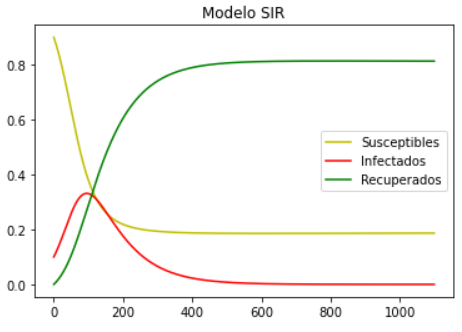
\includegraphics[width=0.4\textwidth]{Imagenes/ex1SIR.PNG}
      \caption{\centering Evolución de la enfermedad en 1100 días con $S_0=0.9,I_0=0.1,R_0=0$ y $h=0.1$.}
      \label{fig:ex1SIS}
    \end{figure}
\end{itemize}